\section{Iterations} 
\subsection{Sprint 1}
\subsubsection{Plan}
In this sprint we aimed to get a simple working version of Blackjack that runs from a GUI. \\

\noindent We added 6 (Main, card, deck, hand, player, and game).java that serves as our business logic for our game. Additionally we added a login screen that allows the user to sign in, create an account, or play as a guest. We have also implemented the base for our backend database that stores our users login info.

\subsubsection{Activities}

\textbf{User Stories Attempted (Beginning of Sprint 1)}

Callie, Chris 
\begin{itemize}
    \item [--] S26 Play Blackjack (3pts) 
    \item [--] S14 Change Ace Value (1pt)
    \item [--] S21 View Tutorial (1pt)
\end{itemize} 
Jenna, Emma
\begin{itemize}
    \item [--] S1 Login (2pts) 
    \item [--] S2 Logout (1pt)
    \item [--] S3 Create Account (2pts)
    \item [--] S7 Play as Guest (2pts)
\end{itemize} 

Total Points Attempted this Sprint: 12\\

\textbf{User stories Accomplished (End of Sprint 1)}
Callie, Chris
\begin{itemize}
    \item [--] S26 Play Blackjack (3pts)
    \item [--] S21 View Tutorial (1pt)
\end{itemize} 
Jenna, Emma
\begin{itemize}
    \item [--] S1 Login (2pts) 
    \item [--] S3 Create Account (2pts)
\end{itemize} 

Total Points Accomplished this Sprint: 8

\begin{table}[!hbt]
\begin{tabular}{|l|l|l|l|}
\hline
\multicolumn{1}{|c|}{\textbf{Name}} & \multicolumn{1}{c|}{\textbf{Speed}} & \multicolumn{1}{c|}{\textbf{Paired Programming}} & \textbf{Individual Cycle (per/hr)} \\ \hline
Callie & 4 & /2 = 2pts & ~35hrs/2pts = 17.5hrs per point   \\ \hline
Chris  & 4 & /2 = 2pts & ~34hrs/2pts = 16hrs per point \\ \hline
Emma   & 4 & /2 = 2pts & ~29hrs/2pts = 14.5hrs per point   \\ \hline
Jenna  & 4 & /2 = 2pts & ~40hrs/2pts = 20hrs per point \\ \hline
\end{tabular}
\end{table}

\subsubsection{Sprint 1 Testing}

Here are the individual testing results for each member/pair:

Chris/Callie:
\begin{figure}[!hbt]
    \centering
    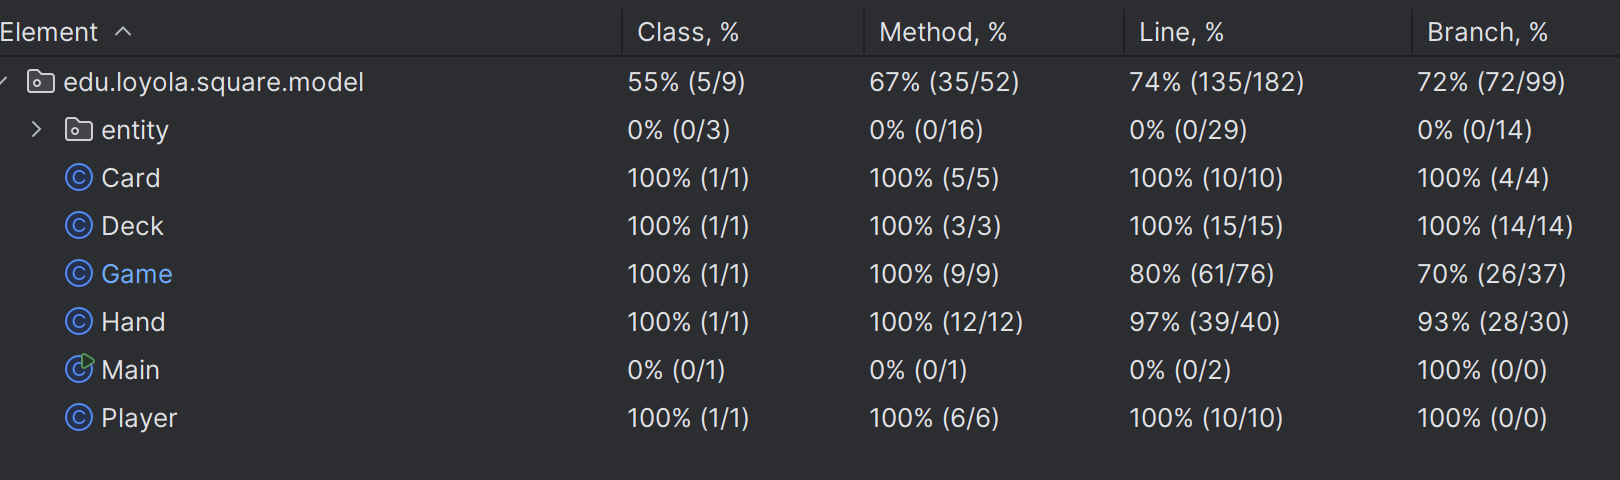
\includegraphics[width=1.0\linewidth]{figures/Coverage report (Model).png}
    \caption{Coverage for Chris/Callie's Code}
    \label{Coverage report}
\end{figure}

Jenna:
\begin{figure}[!hbt]
    \centering
    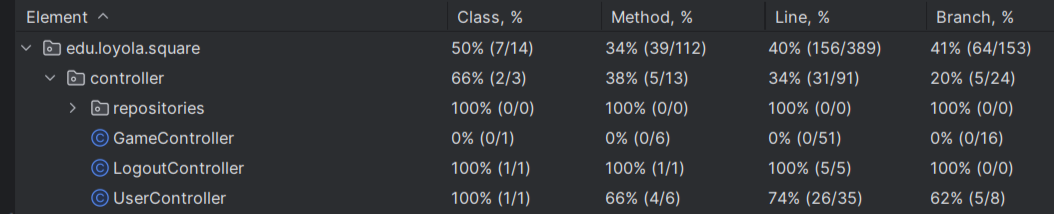
\includegraphics[width=1.0\linewidth]{figures/JennaTest.png}
    \caption{Coverage for Jenna's Code}
    \label{Jenna coverage}
\end{figure}\\


Emma:
\begin{figure}[!hbt]
    \centering
    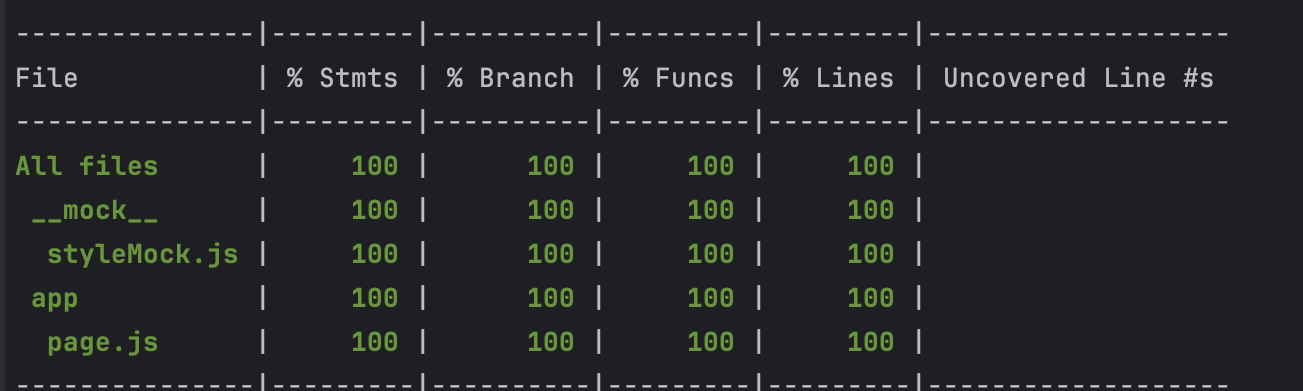
\includegraphics[width=1.0\linewidth]{figures/EmmaTest.png}
    \caption{Coverage for Emma's Code}
    \label{Emma Coverage}
\end{figure}

Callie:
\begin{figure}[!hbt]
    \centering
    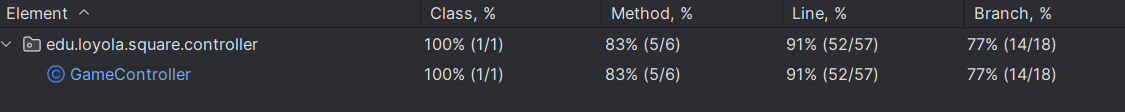
\includegraphics[width=1.0\linewidth]{figures/CallieTest.png}
    \caption{Coverage for Callie's code}
    \label{Callie Coverage}
\end{figure}



\subsubsection{Retrospective}
We realized that integration between model, view and controller can take much more time than anticipated. Additionally, some of our original point values for our user stories might have been underestimated.

%[[ The requirements analysis identifies \textbf{what} your client wants.
%With each iteration describe the \textbf{how}.
%Include user stories attempted, data structures introduced, and any key design
%decisions.

%Copy this layout for each iteration. ]]


